%\begin{figure}[h]
	%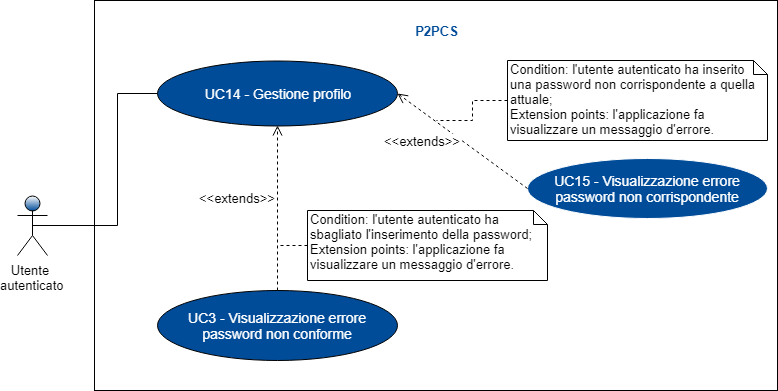
\includegraphics[width=15cm]{res/images/Schemagenerale5.png}
	%\centering
	%\caption{Schema generale: gestione profilo ed errori annessi}
%\end{figure}


\subsubsection{UC20 - Milestone Unlock}
\begin{itemize}
	\item \textbf{Attori Primari}: utente autenticato;
	\item \textbf{Descrizione}: L'utente generico può visualizzare la tabella Milestone Unlock\glo, che illustra per ogni livello esperienza il corrispettivo premio che si può ottenere;	
	\item \textbf{Scenario principale}: l'utente ha premuto il pulsante per la visualizzazione della tabella Milestone Unlock, e la sta visualizzando.
	I premi presenti nella tabella possono essere del seguente tipo:
	\begin{itemize}
		\item aumento del valore del prossimo buono sconto che si andrà a ricevere (x\% in più);
		\item sconto dell'x\% sul prossimo acquisto nel negozio dell'applicazione;
		\item beni virtuali.
	\end{itemize}
	I premi partono dal quinto livello esperienza.
	Ogni 10 livelli esperienza, il valore del premio è aumentato del 10\%.
	\item \textbf{Precondizione}: l'utente autenticato ha premuto il pulsante della Milestone Unlock, dal menu dell'applicazione;
	\item \textbf{Postcondizione}: l'utente autenticato sta visualizzando la tabella Milestone Unlock;
	\item \textbf{Estensioni}:
			l'utente autenticato ha raggiunto un nuovo livello esperienza e ritira il premio corrispondente al livello raggiunto tramite la tabella Milestone Unlock [UC21].
\end{itemize}
\subsubsection{UC21 - Ritiro premio per raggiungimento nuovo livello esperienza}
\begin{itemize}
	\item \textbf{Attori Primari}: utente autenticato;
	\item \textbf{Descrizione}: L'utente autenticato ha raggiunto un nuovo livello esperienza presente nella tabella Milestone Unlock\glosp e può ritirare il relativo premio;	
	\item \textbf{Scenario principale}: l'utente autenticato ha raggiunto un nuovo livello esperienza e gli si presenta la tabella di Milestone Unlock, dalla quale può ritirare il corrispondente premio. Il premio appena sbloccato sarà illuminato da un'aura gialla.
	\item \textbf{Precondizione}: l'utente autenticato ha raggiunto un nuovo livello esperienza, superiore al 5.
	\item \textbf{Postcondizione}: l'utente autenticato può ritirare il premio corrispondete al livello raggiunto, tramite la tabella Milestone Unlock.
\end{itemize}
